\documentclass[../Head/Main.tex]{subfiles}
\begin{document}
\subsection{Test of marble detection on camera data}
\label{subsec:test_cv_marble}
The purpose of this test was to test the performance of the marble detecting method on different scenarios of camera data.
\subsubsection*{Description of test}
In this test a total of 5 tests was conducted to see the performance of the method in different cases. The tests was conducted by first separation the marbles from the background using the method \texttt{find\_color()}, and the run the marble detection method on the binary image.	

\subsubsection*{Data}
In figure (\ref{fig:md_1}) a single marble can be seen, without another marble being visible behind it or being blocked a wall. This marble was detected without any errors, meaning that the marble detecting method works very well in this case.\\
In figure (\ref{fig:md_2}) two marbles can be seen, one further into the distance and behind the first closer marble. In this case the methods only detects a single marble consistent with the closer marble, but the center slightly shifted to the right, due to the methods inability do distinguish the two marbles. In this case direction to the marble would be slightly off, which could lead to the robot missing the marble.\\   
\begin{figure}[H]
	\centering
	\begin{subfigure}[b]{0.45\textwidth}
		\centering
		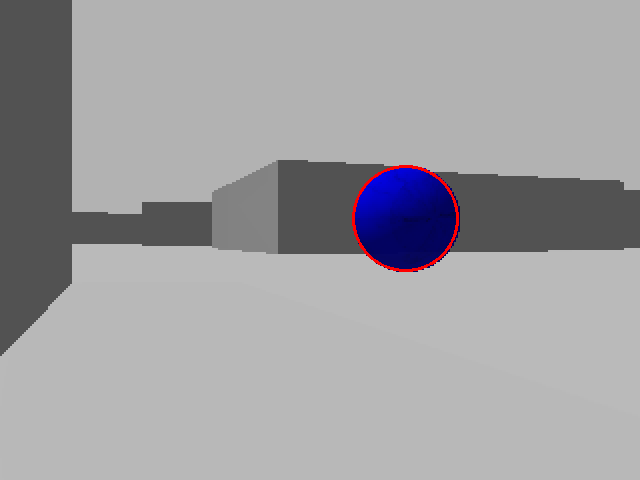
\includegraphics[width=\textwidth]{CV/camera_detected_marbles_2}
		\caption{Marble detection on scenario 1}
		\label{fig:md_1}
	\end{subfigure}
	\hfill
	\begin{subfigure}[b]{0.45\textwidth}
		\centering
		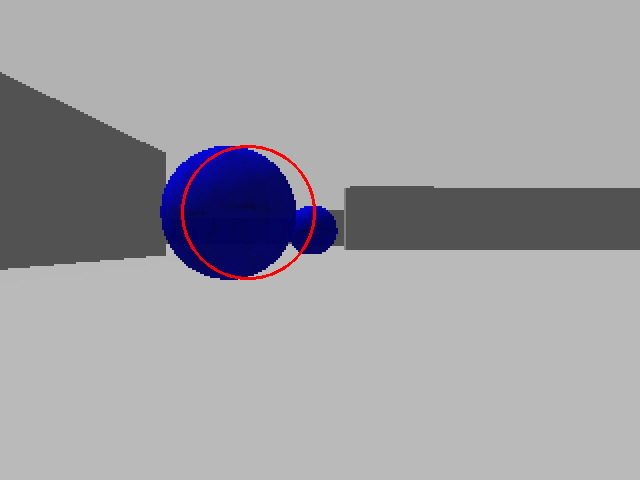
\includegraphics[width=\textwidth]{CV/camera_detected_marbles_3}
		\caption{Marble detection on scenario 2}
	\end{subfigure}
	\caption{Marble detection of scenario 1 and 2}
	\label{fig:md_2}
\end{figure}

In figure (\ref{fig:md_3}) two marbles can be seen, on further away than the other. There are no overlap between the two marbles resulting in good detection of both marbles.\\
In figure (\ref{fig:md_4}) a single very close marble can be seen. It can be seen that the detected marble has a smaller radius than the actual marble, due to the fact that a part of the marble are out of the image. This means that center of the marble are shifted slightly downwards.
\begin{figure}[H]
	\centering
	\begin{subfigure}[b]{0.45\textwidth}
		\centering
		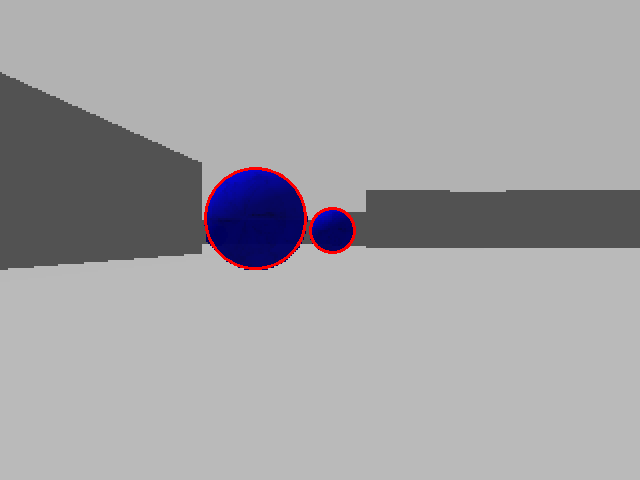
\includegraphics[width=\textwidth]{CV/camera_detected_marbles_4}
		\caption{Marble detection on scenario 3}
		\label{fig:md_3}
	\end{subfigure}
	\hfill
	\begin{subfigure}[b]{0.45\textwidth}
		\centering
		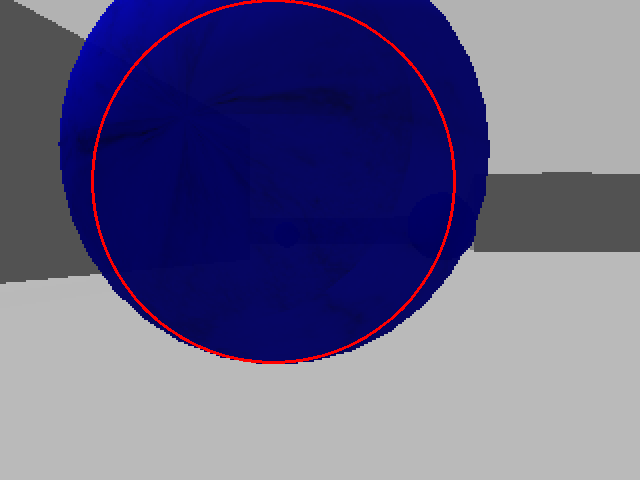
\includegraphics[width=\textwidth]{CV/camera_detected_marbles_5}
		\caption{Marble detection on scenario 4}
		\label{fig:md_4}
	\end{subfigure}
	\caption{Marble detection of scenario 3 and 4}
\end{figure}

In figure (\ref{fig:md_5}) two marbles can be seen, one slightly covered by a wall, and the other slightly in the image. Both marbles was detected correctly. The closet one with a slightly off radius and the one further away with a slightly off center. 
\begin{figure}[H]
	\centering
	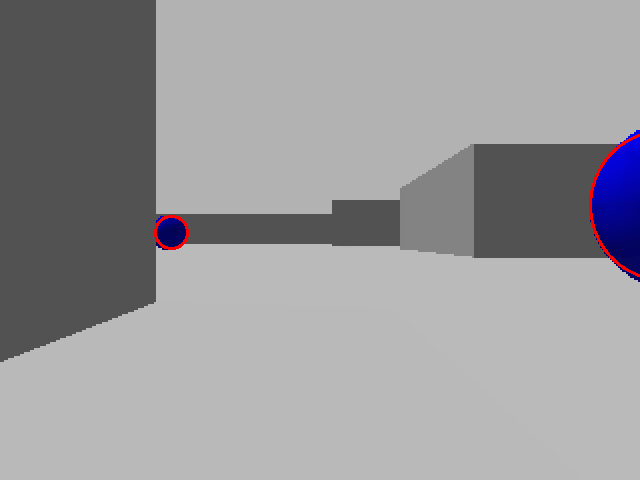
\includegraphics[width=0.45\textwidth]{CV/camera_detected_marbles_6}
	\caption{Marble detection on scenario 5}
	\label{fig:md_5}
\end{figure}

\subsubsection*{Conclusion}
It can be concluded that the marble detecting method works great if the entire marble are visible in the image without another marble hiding behind it. If another marble was to be seen behind the first, it can be concluded that the center would be shifted towards the marble further away. \\
It can be concluded that marbles cut off on either the left or the right side would be detected correctly, but might have slightly off center and radius.\\
It can be concluded that a marble cut off on either the top or the bottom would result in incorrectly  radius. The center would be placed correctly on the x-axis and off on the y-axis. 

\end{document}